For the final Milestone, each group member was required to individually implement different Barrelfish subsystems and then jointly integrate them at the end. This chapter delves into the \textit{nameserver} and was completed by \textbf{Mathew}.
\\\\
Due to time constraints I was not able to get this Milestone done, so this chapter is written from a ``what if" perspective. All design here is theoretical and may gloss over some finer details that only would have been revealed during the implementation process.

\subsection{Introduction}
Up until this point, we have been writing services for our operating system that are hardcoded into the RPC library. For example, in order for a user process to communicate with the process management server, it needs to make a call to \texttt{aos\_rpc\_get\_process\_channel}. If it wants to get the status of a process, it then needs to make a call to \texttt{aos\_rpc\_proc\_get\_status}. This is not sustainable and somewhat antithetical to the idea of the microkernel, so we set out in this chapter to implement a ``nameserver". The nameserver, in theory, acts as a mediator between clients and services. For example, a service should be able to register itself under a unique name with the nameserver, and a client should then be able to query the nameserver and receive a handle for communicating with the service.

\subsection{Design Constraints}
The nameserver will have to handle a steady amount of requests over time since it is possible for hundreds of processes to simultaneously be running on our operating system. We can expect a fair amount of these processes to make at least one or two requests to the nameserver so as to either register a service or look one up. On that note, we also want to think about how the nameserver should structure its data since it must hold mappings between registered service names and their connection data. I identified the following challenges with respect to the nameserver implementation:
\begin{itemize}[itemsep=0pt]
    \item How does binding work? The nameserver needs to do some routing so that an arbitrary client and service can connect to each other.
    \item How should the nameserver store its service data?
    \item Which services should the nameserver return when responding to a search request?
    \item How does a service deal with multiple client connections?
    \item Should the nameserver run on the monitor or in its own process?
    \item How do nameservers on different cores coordinate with each other?
\end{itemize}

\subsection{Possible Implementations}
We need to start off by thinking about where the nameserver will \textit{live}. Assuming that we want to use UMP for binding requests (which would be ideal since it's faster than LMP), the monitor will somehow have to be involved in order to transfer capabilities across cores. This leaves us with two options, the first being to simply run all nameserver functionality on the monitor (Figure \ref{figure:nameserver}). RPCs to the nameserver in this case would require a minimal amount of IPC and the implementation effort would be straightforward, but the design is less faithful to the Single Responsibility Principle.
\begin{figure}[ht]
    \centering
    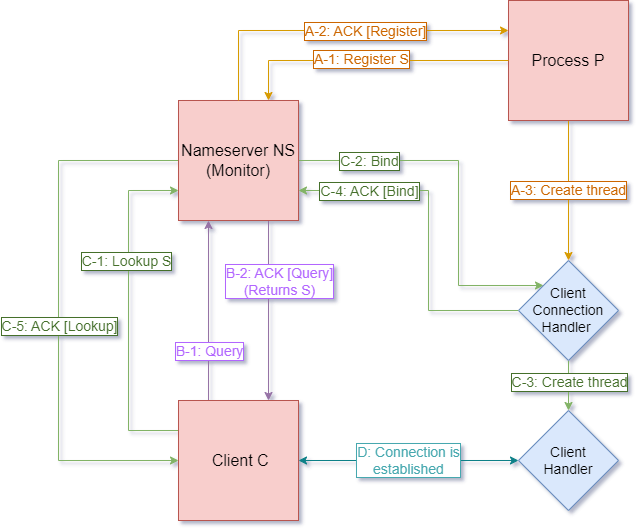
\includegraphics[width=0.5\columnwidth]{images/nameserver.png}
    \caption{Call graph for a nameserver running on the monitor.}
    \label{figure:nameserver}
\end{figure}
\\\\
The second option involves distinguishing between \textit{naming} and \textit{binding} (Figure \ref{figure:bindingserver}). In this case, the nameserver runs in its own process and stores a mapping between service names and their channels. The ``binding server" is the monitor, and is communicated with whenever the nameserver needs to create a connection (either between itself and a service, or between a client and a service). This approach is nice because not all cases where processes want to bind with each other make sense as a ``service". In these cases, they simply make an RPC to the binding service and don't have to worry about advertising themselves to the nameserver. This separation of concerns adds some overhead however, as more RPCs are necessary for the nameserver to handle binding. 
\begin{figure}[ht]
    \centering
    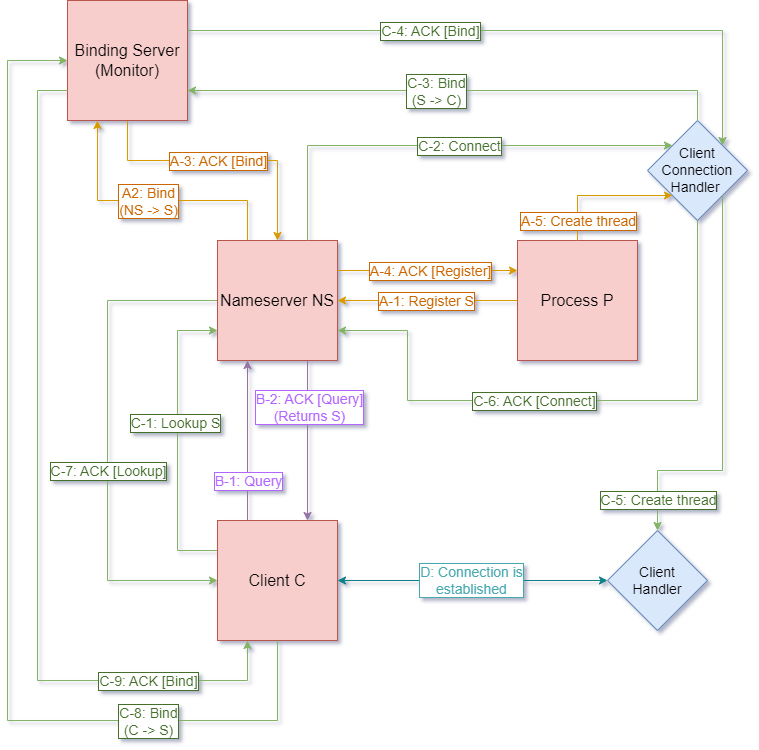
\includegraphics[width=0.5\columnwidth]{images/bindingserver.png}
    \caption{Call graph for a nameserver running outside of the monitor.}
    \label{figure:bindingserver}
\end{figure}
\\\\
As mentioned previously I did not actually implement anything, so in the spirit of taking the easier approach we assume the nameserver runs on the monitor (option 1) for the rest of this chapter. Also assume that like before, all new processes spawn with a connection to the monitor (running the nameserver). This is the only connection necessary since all other services can be accessed using it.

\subsubsection{Registration}
A process \textbf{P} registers a service \textbf{S} with the nameserver \textbf{NS}:
\begin{enumerate}[itemsep=0pt]
    \item \textbf{P} sends a \texttt{register} request to \textbf{NS} containing an identifier for \textbf{S}, and a UMP/LMP capability to itself.
    \item \textbf{NS} creates a connection to \textbf{P} using the capability, stores a mapping between \textbf{S} and the connection, and returns an ACK.
    \item \textbf{P} creates its side of the connection and spawns a thread to listen on it. The thread is set up with a message handler that handles new client connection requests. We will refer to this thread as the ``client connection handler" (\textbf{CCH}).
    \item \textbf{P} stores a mapping between the service handler (the function that will be used to respond to clients) and the identifier for \textbf{S}. This handler will run on a thread when a new client connects. We can expect \textbf{P} to run a small number of services, so a linked list will suffice here. A hash table would be marginally faster (on average), but I figured that if I were to have completed this Milestone, I would have saved myself the headache.
\end{enumerate}
Note that under this scheme, one process may run multiple services (each service having its own connection handler thread). Also note that the client connection handler allows a service to serve multiple clients (this is explained in detail later).

\subsubsection{Queries}
When a client wants to ``search" for registered services, it makes an \texttt{enumerate} request to the nameserver. This breaks down into two problems: what data structure does the nameserver use to store service mappings, and what string-searching algorithm does it implement to find those mappings when queried? The search problem also ties in with naming, since it depends on what exactly processes provide as a name when registering a service. It would be a bit overkill at this point to introduce sophisticated naming/search schemes since we only have a few services running, so for now we assume that names may only consist of alphanumeric characters, and that queries return all names containing the search string as a subset. More formally, given a set of names $N$ and a search string $s$, we return all names $n \in N$ such that $s \subseteq n$.
\\\\
The string-search algorithm we implement places limitations on how mappings are stored. A hash table would be very nice here since it fits our need of quick lookups, insertions, and deletions, however using one necessitates that when queried we only return names that exactly match the search string. This would effectively turn \texttt{enumerate} into a ``service exists?" request, which is less than ideal. Instead, we opt for a linked list. Registrations become constant-time (we can just insert at the front/back), while deletions/lookups suffer a bit and turn into linear-time operations, since we have to search the list for anything matching our search string. A case can be made that this is fine since we're not expecting a massive number of services, however an analysis of the ``average case" would be needed to back that claim, and linked lists don't mesh too well with cache/memory since each access requires a pointer-hop. While thinking about this I realized that an abstract syntax tree would solve some of these issues, however I figured that I ultimately would have went with the linked list due to its simplicity.

\subsubsection{Lookup}
A client \textbf{C} asks the nameserver \textbf{NS} for a connection to a service \textbf{S} (running on \textbf{P}):
\begin{enumerate}[itemsep=0pt]
    \item \textbf{C} sends a \texttt{lookup} request to \textbf{NS} containing the name of \textbf{S}, and a UMP/LMP capability to itself.
    \item \textbf{NS} sends a ``bind`` request to \textbf{S}, which is caught by its client connection handler \textbf{CCH}.
    \item \textbf{CCH} creates its side of the connection and spawns a thread \textbf{CH} to listen on it. The thread is set up to run the service handler that \textbf{P} stored during the registration process.
    \item \textbf{CCH} returns an ACK to \textbf{NS}, which returns an ACK to \textbf{C}.
    \item \textbf{C} creates its side of the connection and can now talk with \textbf{P}. Requests from \textbf{C} are caught and responded to by \textbf{CH}. 
\end{enumerate}

\subsection{Multicore Support}
The final issue we have to deal with is multicore support. Since each core has its own monitor, and the nameserver \textit{is} the monitor, we need a way to synchronize their service lists. When a service registers with the nameserver, we need to decide if we want to notify the other core immediately, or hold off until a request comes in that requires the aggregate list (e.g. \texttt{enumerate}). Ideally, we want to pick a design that minimizes the amount of IPC happening.
\\\\
If we decide \textit{not to notify} the other core immediately, the nameserver needs to query it before serving \texttt{enumerate}, \texttt{lookup}, and \texttt{deregister} requests. \texttt{enumerate} is relatively easy to implement since we just have to make another \texttt{enumerate} request to the other core and then concatenate the list before serving the request. \texttt{lookup} also requires us to make an \texttt{enumerate} request to the other core, if the nameserver serving the request does not find the service in its local list. If it doesn't, it must make a cross-core binding request (we have an implementation for this from Milestone 6). Finally, \texttt{deregistration} under this design requires cross-core calls no matter what. Since services may be distributed (e.g. process management), the nameserver needs to make another \texttt{deregister} call to the other core. Similar to Milestone 6, we need to be careful about infinite loops in \texttt{enumerate} and \texttt{deregister} since these calls get propagated to the sister core (setting a flag in the request works here).
\\\\
If we decide \textit{to notify} the other core immediately, the nameserver needs to talk to the other core during \texttt{register} and \texttt{deregister} requests. I would have chosen this design because we can always expect exactly 1 \texttt{register} and 1 \texttt{deregister} to happen per service, but we can't be sure how many \texttt{lookup} and \texttt{enumerate} requests might happen for a given client (which are less costly operations using this design). With this design, note that the nameserver must know what core its stored services are on in order for \texttt{deregister} and \texttt{lookup} to work (so that it knows whether or not to forward these calls).
